\documentclass[tikz,border=7pt]{standalone}
\begin{document}
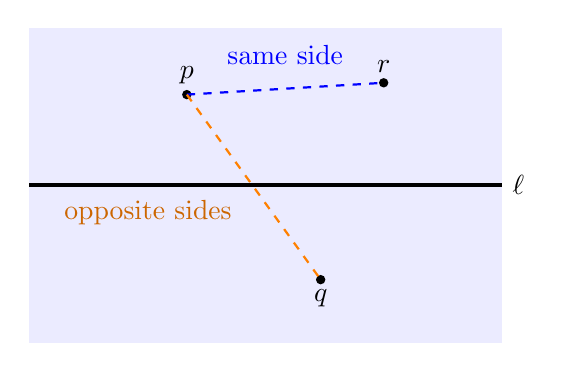
\begin{tikzpicture}[line width=.8pt]
\fill[blue!8] (-3,-2) rectangle (3,2); \draw[very thick] (-3,0)--(3,0) node[right] {$\ell$};
\fill (-1,1.15) circle (1.7pt) node[above] {$p$}; \fill (1.5,1.3) circle (1.7pt) node[above] {$r$}; \fill (.7,-1.2) circle (1.7pt) node[below] {$q$};
\draw[blue,dashed] (-1,1.15)--(1.5,1.3); \node[blue] at (.25,1.65) {same side};
\draw[orange,dashed] (-1,1.15)--(.7,-1.2); \node[orange!80!black,left] at (-.3,-.35) {opposite sides};
\end{tikzpicture}
\end{document}
